\chapter{PHÂN TÍCH YÊU CẦU HỆ THỐNG}

\section{Xác định tác nhân (Actors)}
Trong hệ thống website cung cấp dịch vụ Cloud, có hai tác nhân chính tham gia tương tác với hệ thống:
\begin{itemize}
    \item \textbf{Khách hàng (Customer):} Là người dùng truy cập vào website để xem thông tin dịch vụ, so sánh bảng giá, đặt mua dịch vụ (VPS, Hosting, Domain, v.v.) và đăng ký trở thành đối tác liên kết (Affiliate).
    \item \textbf{Quản trị viên (Admin/Editor):} Là nhân viên của công ty cung cấp dịch vụ, có nhiệm vụ cấu hình bảng giá, quản lý các danh mục dịch vụ, xử lý/duyệt đơn đặt hàng từ khách hàng, quản lý chương trình khuyến mãi, xuất báo cáo doanh thu và đăng tải bài viết/tin tức. Hệ thống phân quyền thành 2 role: \texttt{Admin} (toàn quyền) và \texttt{Editor} (quyền hạn chế, chỉ quản lý nội dung).
\end{itemize}

\section{Yêu cầu chức năng}

\subsection{Chức năng trang công khai (Landing Page)}
Bảng~\ref{tab:func_public} liệt kê đầy đủ các chức năng của trang công khai mà khách hàng có thể truy cập mà không cần đăng nhập.

\begin{table}[htbp]
    \centering
    \caption{Bảng chức năng trang công khai (Landing Page)}
    \label{tab:func_public}
    \begin{tabular}{|c|p{3cm}|p{9cm}|}
        \hline
        \textbf{STT} & \textbf{Chức năng} & \textbf{Mô tả chi tiết} \\
        \hline
        1 & Trang chủ & Hero banner giới thiệu, hiển thị danh mục dịch vụ nổi bật (lấy từ API), cam kết Uptime 99.99\%, tin tức mới nhất, testimonials khách hàng. \\
        \hline
        2 & Giới thiệu & Lịch sử công ty, hạ tầng datacenter, các chứng chỉ (ISO), cam kết SLA/Uptime 99.99\%, đội ngũ kỹ thuật. \\
        \hline
        3 & Dịch vụ & Danh mục: VPS, Hosting, Domain, Email doanh nghiệp, SSL, Firewall chống DDoS. Mỗi dịch vụ kèm mô tả và thông số kỹ thuật chi tiết. \\
        \hline
        4 & Bảng giá & So sánh các gói theo cấu hình (CPU/RAM/SSD/Băng thông). Chuyển đổi giá theo chu kỳ Tháng/Năm (toggle). Hiển thị mã QR cho từng gói dịch vụ. \\
        \hline
        5 & Khách hàng & Đánh giá/testimonial từ khách hàng, logo đối tác tiêu biểu. \\
        \hline
        6 & Tin tức / Blog & Danh sách bài viết với phân trang, tìm kiếm theo từ khóa, phân loại (hướng dẫn, khuyến mãi). Trang chi tiết bài viết theo slug. \\
        \hline
        7 & Liên hệ / Đặt DV & Form đăng ký: chọn chủ đề dịch vụ, nhập thông tin khách hàng. Dữ liệu được lưu vào Database qua API. \\
        \hline
        8 & Đối tác / Affiliate & Trang thông tin chính sách hoa hồng, danh sách đối tác chiến lược. Form đăng ký làm đối tác/affiliate gửi qua API. \\
        \hline
    \end{tabular}
\end{table}

\subsection{Chức năng trang quản trị (Admin Dashboard)}
Bảng~\ref{tab:func_admin} liệt kê các chức năng quản trị, yêu cầu đăng nhập JWT và phân quyền Role.

\begin{table}[htbp]
    \centering
    \caption{Bảng chức năng trang quản trị (Admin Dashboard)}
    \label{tab:func_admin}
    \begin{tabular}{|c|p{3.5cm}|p{6cm}|p{2.5cm}|}
        \hline
        \textbf{STT} & \textbf{Chức năng} & \textbf{Mô tả chi tiết} & \textbf{Role} \\
        \hline
        1 & Đăng nhập, Refresh Token, Đổi mật khẩu & Xác thực bằng JWT. Hỗ trợ Refresh Token gia hạn phiên và đổi mật khẩu cho tài khoản đang đăng nhập. & Tất cả \\
        \hline
        2 & CRUD Gói dịch vụ & Thêm, sửa, xóa các gói dịch vụ (CPU, RAM, Disk, giá). Tự động cập nhật giá trên trang công khai. & Admin \\
        \hline
        3 & CRUD Danh mục DV + Sinh QR & Quản lý danh mục (VPS, Hosting, Domain). Sinh mã QR cho từng gói, quét ra trang chi tiết. & Admin \\
        \hline
        4 & CRUD Tin tức/Blog & Soạn thảo, chỉnh sửa, xóa tin tức. Hỗ trợ gắn slug URL. & Admin, Editor \\
        \hline
        5 & Quản lý Đơn hàng + Affiliate & Xem danh sách, đổi trạng thái (Mới $\rightarrow$ Đang xử lý $\rightarrow$ Hoàn tất/Từ chối). & Admin, Editor \\
        \hline
        6 & CRUD Khuyến mãi & Thêm, sửa, xóa chương trình khuyến mãi với mã code, phần trăm giảm giá, thời hạn. & Admin \\
        \hline
        7 & Thống kê biểu đồ & Tổng quan: số đơn hàng, doanh thu theo tháng, gói dịch vụ được quan tâm. Biểu đồ trực quan. & Admin \\
        \hline
        8 & Xuất Excel & Xuất danh sách yêu cầu đặt dịch vụ ra file Excel (.xlsx) qua thư viện ClosedXML. & Admin \\
        \hline
        9 & Audit Log & Ghi lại lịch sử: ai đăng nhập, ai sửa giá, khi nào. Hiển thị dạng bảng có phân trang. & Admin \\
        \hline
    \end{tabular}
\end{table}

\section{Yêu cầu phi chức năng}
\begin{itemize}
    \item \textbf{Giao diện (UI/UX):} Website phải có thiết kế hiện đại, tốc độ phản hồi nhanh (dưới 3 giây) và hiển thị tốt trên cả nền tảng Desktop và Mobile (Responsive). Menu điều hướng hỗ trợ Hamburger menu trên thiết bị di động.
    \item \textbf{Bảo mật:} Mật khẩu phải được mã hóa bằng thuật toán BCrypt trước khi lưu trữ. Các API quản trị yêu cầu xác thực JWT nghiêm ngặt với phân quyền theo Role (\texttt{[Authorize(Roles = "Admin")]}).
    \item \textbf{Kiến trúc:} Hệ thống được xây dựng theo mô hình Clean Architecture 4 tầng, đảm bảo tính tách biệt (Separation of Concerns) giữa các module.
    \item \textbf{Tính sẵn sàng và mở rộng:} Hệ thống được đóng gói bằng Docker, chỉ cần một lệnh \texttt{docker compose up} là có thể triển khai trên mọi hệ điều hành.
    \item \textbf{Kiểm thử:} Tối thiểu 15 unit test cases sử dụng xUnit và Moq, đảm bảo tính đúng đắn của logic nghiệp vụ tại tầng Application.
\end{itemize}

\section{Sơ đồ Use Case (Ca sử dụng)}
Sơ đồ Use Case tổng quát giúp hình dung rõ bức tranh toàn cảnh về cách các tác nhân tương tác với hệ thống. Khách hàng (Customer) tương tác với các trang công khai, còn Quản trị viên (Admin/Editor) tương tác với hệ thống quản trị sau khi xác thực JWT.

% TODO: Chèn ảnh Sơ đồ Use Case tổng quát. Hãy lưu file ảnh tên là 'use_case_diagram.png' vào thư mục 'images'
\begin{figure}[htbp]
    \centering
    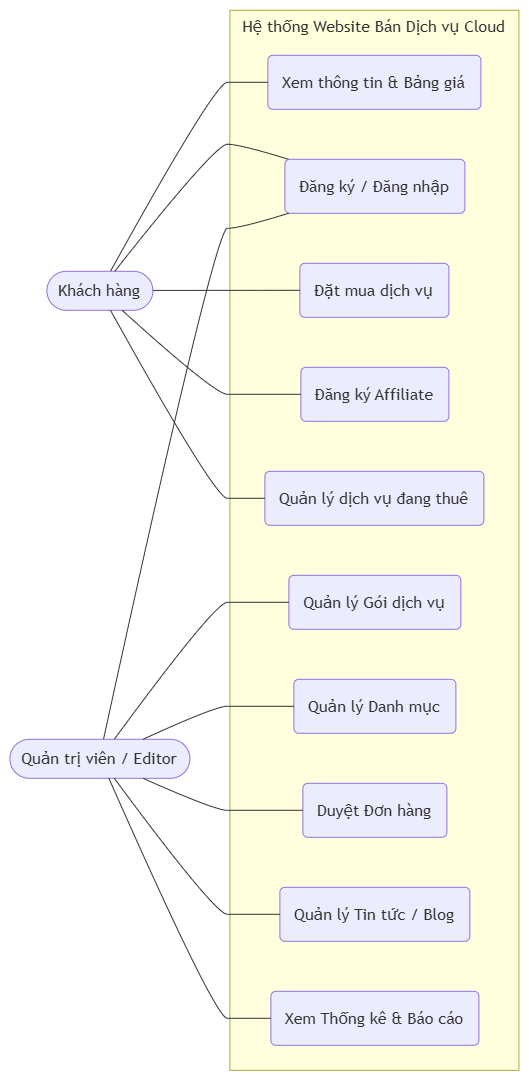
\includegraphics[width=0.7\textwidth]{images/use_case_diagram.png}
    \caption{Sơ đồ Use Case tổng quát của hệ thống Website bán dịch vụ Cloud}
    \label{fig:use_case}
\end{figure}

\section{Sơ đồ Hoạt động (Activity Diagram)}
Để làm rõ luồng nghiệp vụ cốt lõi, Sơ đồ hoạt động sau đây minh họa quy trình ``Đặt hàng dịch vụ'' của một khách hàng từ lúc bắt đầu cho đến khi quản trị viên phê duyệt đơn hàng.

% TODO: Chèn ảnh Sơ đồ Hoạt động Đặt hàng. Hãy lưu file ảnh tên là 'activity_order.png' vào thư mục 'images'
\begin{figure}[htbp]
    \centering
    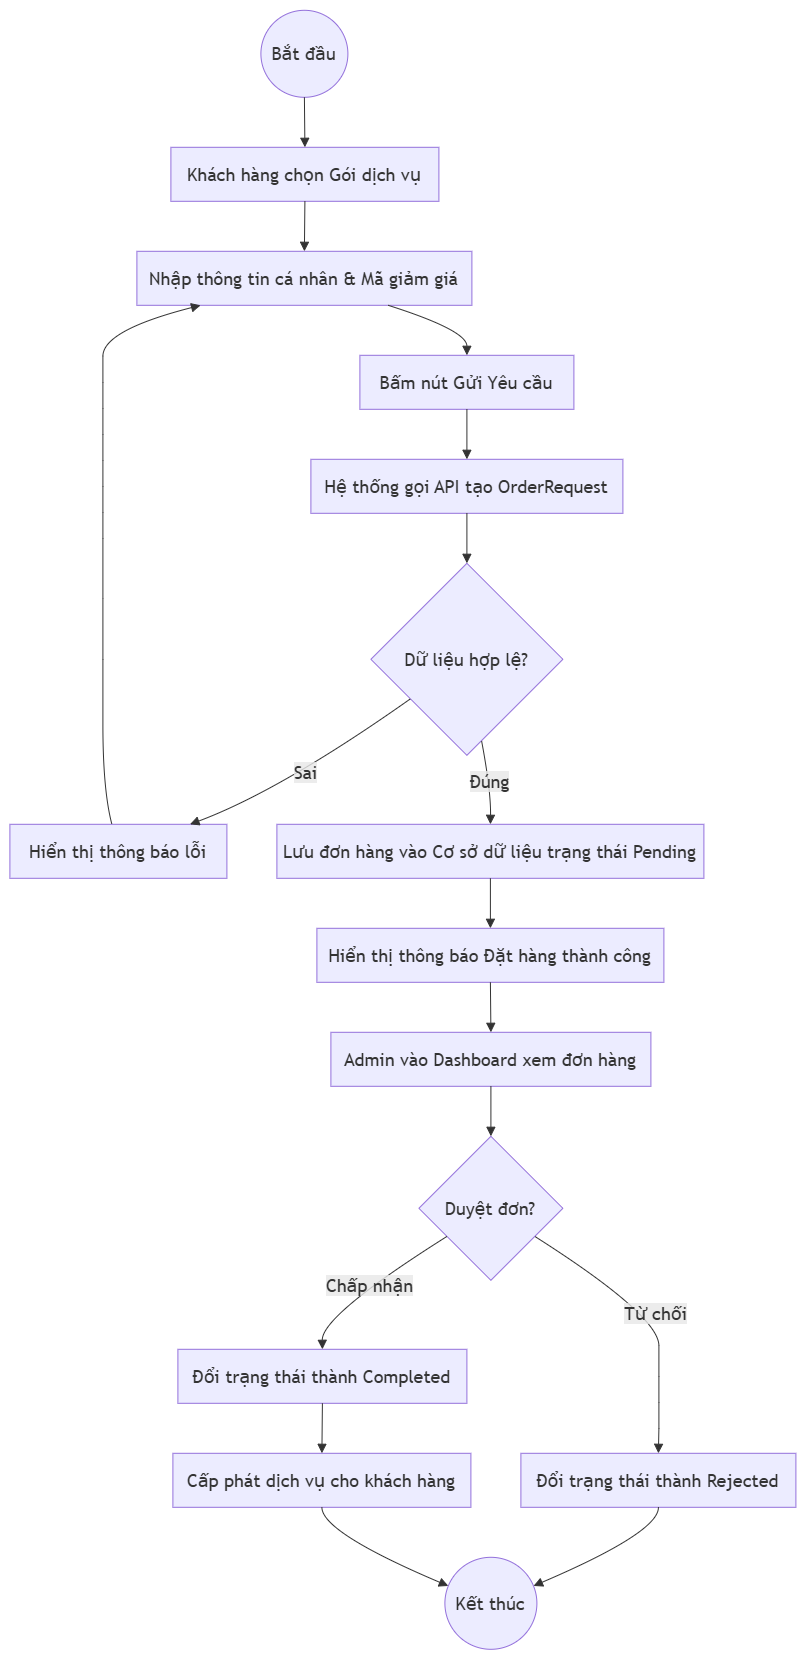
\includegraphics[width=0.7\textwidth]{images/activity_order.png}
    \caption{Sơ đồ Hoạt động nghiệp vụ Đặt hàng dịch vụ}
    \label{fig:activity_order}
\end{figure}
